\documentclass[a4paper]{article} %размер бумаги устанавливаем А4
% \usepackage[T2A]{fontenc}
\usepackage{polyglossia}
\usepackage{url} % добавляем поддержку url-ссылок
\setmainlanguage[babelshorthands=true]{russian} % Язык по-умолчанию русский с поддержкой приятных команд пакета babel
\setotherlanguage{english} % Дополнительный язык = английский (в американской вариации по-умолчанию)
\newfontfamily{\cyrillicfonttt}{Times New Roman}

\usepackage{minted} %пакет для подсветки кода
\usepackage{color}
\usepackage{xcolor} % to access the named colour LightGray
\definecolor{LightGray}{gray}{0.9}
\setdefaultlanguage[forceheadingpunctuation=false]{russian}
% для отступа в первом абзаце
\usepackage{indentfirst} 
\parindent=1.25cm % длина отступа в абзацах
% для продвинутых списков
\usepackage{enumitem} 
\usepackage{amssymb,amsfonts,amsmath,cite,enumerate,float,indentfirst} %пакеты расширений
\usepackage{graphicx}% для вставки картинок
\usepackage{url} % добавляем поддержку url-ссылок
\usepackage{hyperref} % пакет для интеграции гиперссылок
\usepackage{amsmath} % добавляем поддержку математических символов
\usepackage{multirow} % понадобится для создания таблицы с объединенными строками
\usepackage{pdfpages}% Добавление внешних pdf файлов
\usepackage{tocloft}
\renewcommand{\cftsecfont}{\mdseries}
\renewcommand{\cftsecpagefont}{\mdseries}
\cftsetindents{section}{0em}{2em}
\cftsetindents{subsection}{0em}{3em}
\cftsetindents{subsubsection}{0em}{4em}
\renewcommand\cfttoctitlefont{\hfill\normalsize\mdseries}
\renewcommand\cftaftertoctitle{\hfill\mbox{}}
\renewcommand{\cftsecleader}{\cftdotfill{\cftdotsep}}

\usepackage{fontspec}
\setmainfont{Times New Roman} %шрифт 
\graphicspath{{images/}}%путь к рисункам
\usepackage[14pt]{extsizes} % для того чтобы задать нестандартный 14-ый размер шрифта

%\makeatletter
%\renewcommand{\@biblabel}[1]{#1.} % Заменяем библиографию с квадратных скобок на точку:
%\makeatother


\usepackage[tableposition=top]{caption}
\usepackage{subcaption}
\DeclareCaptionLabelFormat{gostfigure}{Рисунок #2}
\DeclareCaptionLabelFormat{gosttable}{Таблица #2}
\DeclareCaptionLabelSeparator{gost}{~–~}
\captionsetup{labelsep=gost}
\captionsetup[figure]{labelformat=gostfigure}
\captionsetup[table]{labelformat=gosttable}
\renewcommand{\thesubfigure}{\asbuk{subfigure}}


\makeatletter

\renewcommand{\section}{\@startsection{section}{1}{0pt}%
                                {-3.5ex plus -1ex minus -.2ex}%
                                {2.3ex plus .2ex}%
{\centering\hyphenpenalty=10000\normalfont\normalsize\mdseries}}

\renewcommand{\subsection}{\@startsection{subsection}{1}{0pt}%
                                {-3.5ex plus -1ex minus -.2ex}%
                                {2.3ex plus .2ex}%
{\centering\hyphenpenalty=10000\normalfont\normalsize\mdseries}}
\renewcommand{\subsubsection}{\@startsection{subsubsection}{1}{0pt}%
                                {-3.5ex plus -1ex minus -.2ex}%
                                {2.3ex plus .2ex}%
{\centering\hyphenpenalty=10000\normalfont\normalsize\mdseries}}
\makeatother


\usepackage{setspace}
% \onehalfspacing % полуторный интервал для всего текста
% или \singlespacing % одиночный интервал для всего текста
% или \doublespacing % двойной интервал для всего текста
\setstretch{1.5} % произвольный интервал

% в тексте
% \begin{onehalfspace}
% фрагмент текста с полуторным межстрочным интервалом
% \end{onehalfspace}
% \begin{doublespace}
% фрагмент текста с двойным межстрочным интервалом
% \end{doublespace}

\sloppy % выравнивание по ширине




%%% Поля и разметка страницы %%%
\usepackage{pdflscape}  % Для включения альбомных страниц
\usepackage{geometry}   % Для последующего задания полей
\geometry{left=3cm}% левое поле
\geometry{right=1.5cm}% правое поле
\geometry{top=2cm}% верхнее поле
\geometry{bottom=2cm}% нижнее поле



\renewcommand{\theenumi}{\arabic{enumi}}% Меняем везде перечисления на цифра.цифра
\renewcommand{\labelenumi}{\arabic{enumi}}% Меняем везде перечисления на цифра.цифра
\renewcommand{\theenumii}{.\arabic{enumii}}% Меняем везде перечисления на цифра.цифра
\renewcommand{\labelenumii}{\arabic{enumi}.\arabic{enumii}.}% Меняем везде перечисления на цифра.цифра
\renewcommand{\theenumiii}{.\arabic{enumiii}}% Меняем везде перечисления на цифра.цифра
\renewcommand{\labelenumiii}{\arabic{enumi}.\arabic{enumii}.\arabic{enumiii}.}% Меняем везде перечисления на цифра.цифра



\newcommand{\imgh}[3]{\begin{figure}[h]\center{\includegraphics[width=#1]{#2}}\caption{#3}\label{ris:#2}\end{figure}}
\newcommand{\imghh}[3]{\begin{figure}[H]\center{\includegraphics[width=#1]{#2}}\caption{#3}\label{ris:#2}\end{figure}}


\usepackage{lastpage}
\usepackage{totcount}
\newcounter{totfigures}
\newcounter{tottables}
\newcounter{totreferences}

\makeatletter
    \AtEndDocument{%
      \addtocounter{totfigures}{\value{figure}}%
      \addtocounter{tottables}{\value{table}}%
	  
      \immediate\write\@mainaux{%
        \string\gdef\string\totfig{\number\value{totfigures}}%
        \string\gdef\string\tottab{\number\value{tottables}}%   

      }%
    }
\makeatother

	

\newcommand{\empline}{\mbox{}\newline}
\newcommand{\likechapterheading}[1]{ 
    \begin{center}
   \MakeUppercase{#1}
    \end{center}
    \empline}



\makeatletter
    \renewcommand{\@dotsep}{2}
    \newcommand{\l@likechapter}[2]{{\@dottedtocline{0}{0pt}{0pt}{#1}{#2}}}
\makeatother
\newcommand{\likechapter}[1]{    
    \likechapterheading{#1}    
    \addcontentsline{toc}{likechapter}{\MakeUppercase{#1}}}


\usepackage{cite} % Красивые ссылки на литературу


%% Список литературы с красной строки (без висячего отступа) %%%
\patchcmd{\thebibliography} %может потребовать включения пакета etoolbox
 {\advance\leftmargin\labelsep}
 {\leftmargin=0pt%
  \setlength{\labelsep}{\widthof{\ }}% Управляет длиной отступа после точки
  \itemindent=\parindent%
  \addtolength{\itemindent}{\labelwidth}% Сдвигаем правее на величину номера с точкой
  \advance\itemindent\labelsep%
 }
 {}{}


\makeatletter
\def\@biblabel#1{#1 }
\makeatother


% настройки цветовой палитры для гиперссылок. Цвета можно на свой вкус выбрать здесь:  https://www.overleaf.com/learn/latex/Using_colours_in_LaTeX
\hypersetup{
    citecolor=gray, % цвет цитирования
    colorlinks=true, 
    linkcolor=black, % цвет для гиперссылок 
    filecolor=magenta, % цвет для ссылок на файл      
    urlcolor=mauve} % цвет для url-ссылок
    \usepackage{listings}

\usepackage{color}
\definecolor{dkgreen}{rgb}{0,0.6,0} 
\definecolor{gray}{rgb}{0.3,0.3,0.3}
\definecolor{mauve}{rgb}{0.42,0,0.92}

	
\begin{document}

\begin{titlepage}
\newpage
\begin{doublespace}
% \doublespacing
% \linespread{1.3} % полуторный интервал
%\setlength\parindent{1.25cm}
\begin{center}
МИНИСТЕРСТВО ОБРАЗОВАНИЯ И НАУКИ \\
РОССИЙСКОЙ ФЕДЕРАЦИИ\\
ФЕДЕРАЛЬНОЕ ГОСУДАРСТВЕННОЕ АВТОНОМНОЕ\\
ОБРАЗОВАТЕЛЬНОЕ УЧРЕЖДЕНИЕ ВЫСШЕГО ОБРАЗОВАНИЯ\\
«САМАРСКИЙ НАЦИОНАЛЬНЫЙ ИССЛЕДОВАТЕЛЬСКИЙ\\
УНИВЕРСИТЕТ ИМЕНИ АКАДЕМИКА С.П. КОРОЛЕВА»	\\
(Самарский университет) \\
\end{center}

\vspace{4em}

\begin{center}
Институт информатики и кибернетики \\ 
\end{center}

\begin{center}
Кафедра лазерных и биотехнических систем \\ 
\end{center}


\vspace{3em}

\begin{center}
{Пояснительная записка к курсовому проекту\\''МОНИТОР АКТИВНОСТИ И ОТСЛЕЖИВАНИЯ ПАДЕНИЯ''}
\end{center}

\vspace{11em}




\newbox{\lbox}
\savebox{\lbox}{\hbox{Корнилин Д.В.}}
\newlength{\maxl}
\setlength{\maxl}{\wd\lbox}
\hfill\parbox{15cm}{
\hspace*{5cm}\hspace*{-5cm}Выполнил студент группы 6364-120304D:\hfill\underline{\hspace{4em}}  \hbox to\maxl{Краснов Д.Г.\hfill}\\
\hspace*{5cm}\hspace*{-5cm}Руководитель проекта:\hfill\underline{\hspace{4em}}  \hbox to\maxl{Корнилин Д.В.\hfill }\\
\hspace*{5cm}\hspace*{-5cm}Работа защищена с оценкой:\hfill\underline{\hspace{4em}}  \hbox to\maxl{ \hfill }\\
}


\vspace{\fill}

\begin{center}Cамара 2023\end{center}

\end{doublespace}
\end{titlepage}
\setcounter{page}{2}% это титульный лист
\begin{sloppypar} % помогает в кириллическом документе выровнять текст по краям
\newpage % Так добавляется  новая страница
\section*{ЗАДАНИЕ} %Объявили начало раздела

Разработать усилитель ЭГС с гальванической развязкой. Элемент развязки – оптрон. Вид модуляции ШИМ. Предусмотреть защиту от помех электрохирургического инструмента и индикатор плохого контакта.


Исходные данные:
\begin{itemize}

	\item[--]Значение ёмкости между силовой линии и телом пациента: С=5 пФ;
	\item[--]Значение ёмкости между телом пациента и землёй: С1 = 200 пФ; 

	\item[--]Диапазон изменения сопротивлений электродов: \delta  Z = 10--100 кОм;

	\item[--]Погрешность измерения во входной цепи: \beta = 0,4\%;
	\item[--]Разность электродных потенциалов: \Delta U = 200 мВ;
			\item[--]Диапазон входных напряжений:\begin{math} U_\textup{вх} = 0,01--0,5 мВ; \end{math}
		\item[--]Полоса пропускания усилителя: \Delta F = 0,01 − 10 Гц;
		
	\item[--]Неравномерность АЧХ в полосе пропускания: \delta = ±5\%;
	\item[--]Диапазон выходных напряжений:\begin{math} U_\textup{вых} = ±10 \textup{В};\end{math}
	\item[--]Напряжение внутренних шумов, приведенных ко входу: \begin{math}U_\textup{ш} = 15 мкВ;\end{math}
	\item[--]Амплитуда помехи от силовой сети на выходе: \begin{math}U_\textup{п} = 150 мВ;\end{math}
	\item[--]Длина кабеля отведений: L = 2,5 м;
	\item[--]Емкость кабеля на единицу длины: \begin{math}C_\textup{к} = 20 \textup{пФ}\/\textup{м};\end{math}
	
	
	
	
	\item[--]Емкость изоляции: С_\textup{из}  = 15 пФ;
	\item[--]Сопротивление изоляции: С_\textup{из} = 10×10^{10}  Ом.


\end{itemize}
\end{sloppypar}







% это задание
\begin{sloppypar} % помогает в кириллическом документе выровнять текст по краям
\newpage % Так добавляется  новая страница
\section*{РЕФЕРАТ} %Объявили начало раздела

Пояснительная записка: \pageref*{LastPage}~страниц, \totfig~рисунков, источников, 1 приложение.\\

 % \tottab~таблиц...
 
 
 
ГЛЮКОЗА, УСТРОЙСТВО СЧИТЫВАНИЯ ДАННЫХ, МИКРОКОНТРОЛЛЕР, BLUETOOTH, STM32WB55RCV6


В курсовом проекте разработаны структурная и принципиальная схемы устройства считывания данных для непрерывного мониторинга уровня глюкозы, осуществлен выбор микроконтроллера c интегрированным блоком Bluetooth и АЦП. Разработан алгоритм анализа данных и реализующая его программа на языке Си.

% возможно добавим еще каких то фраз

\end{sloppypar}
% это реферат
\newpage
\renewcommand{\contentsname}{СОДЕРЖАНИЕ}
{\renewcommand{\baselinestretch}{1.5} %интервал для содержания
\tableofcontents
       
}% это содержание
\begin{sloppypar} % помогает в кириллическом документе выровнять текст по краям
\newpage % Так добавляется  новая страница
\section*{ВВЕДЕНИЕ} %Объявили начало раздела
Диабет превратился в одну из основных эпидемий здравоохранения современной эпохи. Ожидается, что во всем мире общее число людей с диабетом вырастет со 171 миллиона в 2000 году до 366 миллионов в 2030 году.\cite{ADXL}

Мало того, что диабет был шестой по значимости причиной смерти, указанной в свидетельствах о смерти в США в 2020 году, но предполагаемая стоимость диабета в Соединенных Штатах в 2002 году составила 132 миллиарда долларов, включая как прямые, так и косвенные расходы (инвалидность, инвалидность, потеря работы, преждевременная смертность).

Известно, что строгий гликемический контроль снижает разрушительные и дорогостоящие вторичные микро- и макрососудистые осложнения, связанные с диабетом, тем самым улучшая качество жизни миллионов пациентов с диабетом и значительно сокращая расходы на здравоохранение. Также, строгий контроль уровня глюкозы обеспечивает клинические преимущества у пациентов в критическом состоянии.

В данном курсовом проекте  рассматривается способ создания устройства на базе микроконтроллера, который сможет отслеживать уровень глюкозы в крови человека.  В процессе были подобраны необходимые в задании микроконтроллер с интегрированным модулем Bluetooth, акселерометр, а также написана управляющая программа на языке Си. 



\end{sloppypar}
% это введение
\begin{sloppypar} % помогает в кириллическом документе выровнять текст по краям
\newpage % Так добавляется  новая страница
\section{РАЗРАБОТКА СТРУКТУРНОЙ СХЕМЫ УСТРОЙСТВА} %Объявили начало раздела
Структурная схема устройства представлена на рисунке \ref{ris:Figures/struct.png}.
\imghh{150mm}{Figures/struct.png}{Структурная схема устройства}

Принцип работы устройства заключается в следующем. Трёхосевой акселерометр фиксирует ускорение по каждой из осей движения. Эти данные поступают в микроконтроллер, где  проходят первичную обработку, и с помощью алгоритма на языке Си анализируются. В результате анализа можно выяснить характер движения человека, и то,  происходит ли падение. 


Так же, данные передаются по модулю Bluetooth, интегрированному в микроконтроллер. На устройстве есть LED-индикатор, который сигнализирует о передаче пакета данных. 

Все элементы схемы питаются от блока питания, который представляет собой литиевый аккумулятор, имеющий номинальное напряжение 3.7 В, и DC-DC преобразователя, который необходим для стабилизации напряжения на уровне 3.3 В, необходимого всем элементам устройства.

\end{sloppypar}
% это раздел структурной схемы
\begin{sloppypar} % помогает в кириллическом документе выровнять текст по краям
\newpage % Так добавляется  новая страница
\section{РАЗРАБОТКА ПРИНЦИПИАЛЬНОЙ СХЕМЫ УСТРОЙСТВА} %Объявили начало раздела
Электрическая принципиальная схема представлена в приложении.

\subsection{Разработка(надо придумать заголовок)}

Для получения кардиосигнала возможны несколько подходов - проектирование собственных схемотехнических решений на основе дискретных компонентов, или использование \acf{AFE} микросхем, например, ADS1293  от Texas Instruments.

Микросхема ADS1293 предназначена для измерения биопотенциалов, в таких медицинских приборах, как портативные электрокардиографы с батарейным питанием, холтеровские мониторы и аппаратура беспроводного мониторинга пациентов. \cite{ADS1293}

ADS1293 способна поддерживать от одного до пяти каналов, что позволяет существенно сократить габариты, энергопотребление и полную стоимость масштабируемых измерительных медицинских систем. Каждый канал ADS1293 может быть независимо запрограммирован на работу со специальными (отличными от других) частотой выборки и полосой пропускания. 

На основании анализа функциональных возможностей и технических характеристик \ac{AFE} ADS1293, можно сделать вывод о том, что кроме очевидных преимуществ по габаритам в сравнении с аналоговой частью холтеровских мониторов на дискретных операционных усилителях (\acs{OU}) и аналого-цифровых преобразователях (\acs{АЦП}), гибридная \ac{IS} обладает достаточно низким энергопотреблением даже в активном режиме, высоким соотношением сигнал/шум и достаточным динамическим диапазоном для решения задач холтеровского мониторирования. Как следствие высокой интеграции аналоговой части и \ac{АЦП}, а так же цифровой подсистемы первичной обработки квантованного сигнала использование \ac{AFE} позволило существенно упростить схемные решения монитора \acs{ЭКГ}, уменьшить габариты и продолжительность автономной работы от батареи той же емкости. 




















Структурная схема акселерометра из даташита ADS1293 \cite{DS1293} приведена на рисунке \ref{ris:Figures/ads1293.png}.

\imghh{160mm}{Figures/ads1293.png}{Структурная схема ADS1293}

Оцифрованный аналоговый сигнал от ADS1293 передается микроконтроллеру поcредством \acf{SPI}.

% Схема подключения представлена на рисунке \ref{ris:Figures/spi.png}.


% \imghh{100mm}{Figures/spi.png}{Cхема подключения ADS1293 к микроконтроллеру по SPI}}


Так же, в даташите приведена рекомендованная схема включения для трехэлектродной схемы(рисунок \ref{ris:Figures/ads1293_connect.png}).

\imghh{160mm}{Figures/ads1293_connect.png}{Трехэлектродная схема включения}



Нумерация и назначение выводов ADS1293 приведены ниже (рисунки \ref{ris:Figures/ads1293_io.png}, \ref{ris:Figures/ads1293_io2.png}).
\imghh{90mm}{Figures/ads1293_io.png}{Нумерация выводов}
\imghh{160mm}{Figures/ads1293_io2.png}{Назначение выводов}




 
% здесь налить водички про то почему был выбрана ADS1293


\subsection{Выбор микроконтроллера}
С учетом технического задания микроконтроллер должен обладать следующими свойствами:
\begin{onehalfspace}
	\begin{itemize}
		\item[--]Интерфейс для работы с микросхемой ADS1293: SPI;
		\item[--]Интерфейс для работы с внешней флеш-памятью: SPI или $I^2$C;
		\item[--]Для передачи данных по Bluetooth: встроенный стек протокола Bluetooth;
		\item[--]Малое энергопотребление;
		\item[--]Свободные выводы для подключения индикатора и выводов прерываний от ADS1293;
	\end{itemize}
\end{onehalfspace}

Для решения задачи был выбран микроконтроллер STM32WB55RCV6 фирмы ST Microelectronics \cite {STM}.STM32WB55 содержит два производительных ядра ARM-Cortex:
\begin{onehalfspace}
	\begin{itemize}
		\item[--] ядро ARM® -Cortex® M4 (прикладное), работающее на частотах до 64 МГц, для пользовательских задач имеется модуль управления памятью, модуль плавающей точки, инструкции ЦОС (цифровой обработки сигналов), графический ускоритель (ART accelerator);
		\item[--] ядро ARM®-Cortex® M0+ (радиоконтроллер) с тактовой частотой 32 МГц, управляющее радиотрактом и реализующее низкоуровневые функции сетевых протоколов;
	\end{itemize}
\end{onehalfspace}

Данный микроконтроллер включает в себя все необходимые периферийные устройства, такие как интерфейсы передачи данных SPI,необходимый для подключения к акселерометру, и радиоконтроллер с поддержкой Bluetooth.

Основные характеристики:
\begin{onehalfspace}
	\begin{itemize}
		\item[--] типовое энергопотребление 50 мкА/МГц (при напряжении питания 3 В);
		\item[--] потребление в режиме останова 1,8 мкА (радиочасть в режиме ожидания (standby));
		\item[--] потребление в выключенном состоянии (Shutdown) менее 50 нА;
		\item[--] диапазон допустимых напряжений питания 1,7…3,6 В (встроенный DC-DC–преобразователь и LDO-стабилизатор);
		\item[--] рабочий температурный диапазон -40…105°С.
	\end{itemize}
\end{onehalfspace}


Структурная схема микроконтроллера приведена на рисунке \ref{ris:Figures/stm32.png}, а назначение выводов портов корпуса на рисунке \ref{ris:Figures/stm32io.png}.

\imghh{90mm}{Figures/stm32io.png}{Назначение выводов}


\imghh{110mm}{Figures/stm32.png}{Структурная схема}


Подключение будет осуществляться согласно типовой схеме из Application note\cite {STM_an}(рисунок \ref{ris:Figures/stm32an.png}).
\imghh{160mm}{Figures/stm32an.png}{Типовая схема подключения STM32WB55}







\begin{sloppypar} % помогает в кириллическом документе выровнять текст по краям


\subsection{Выбор встроенного носителя}
 В качестве носителя информации выберем последовательную FLASH-память серии W25Q \cite{W25Q}. Данная последовательная память может быть различной ёмкости — 8, 16, 32, 64, 128, 256 Мбит и т. д. Подключается такая память по интерфейсу SPI, а также по многопроводным интерфейсам Dual SPI, Quad SPI и QPI. Мы же пока будем подключим данную микросхему по обычному интерфейсу SPI.

Краткие основные характеристики W25Q:

\begin{onehalfspace}
	\begin{itemize}
		\item[--]Потребляемая мощность и температурный диапазон:
		\item[--]Напряжение питания 2.7…3.6 В
		\item[--]Типичный потребляемый ток: 4 мА (активный режим), <1 мкА (в режиме снижения мощности)
		\item[--]Рабочий температурный диапазон -40°C…+85°C.
	\end{itemize}
\end{onehalfspace}

Гибкая архитектура с секторами размером 4 кбайт:
\begin{onehalfspace}
	\begin{itemize}
		\item[--]Посекторное стирание (размер каждого сектора 4 кбайт)
		\item[--]Программирование от 1 до 256 байт
		\item[--]До 100 тыс. циклов стирания/записи
		\item[--] 20-летнее хранение данных
	\end{itemize}
\end{onehalfspace}


Максимальная частота работы микросхемы:
\begin{onehalfspace}
	\begin{itemize}
		\item[--]104 МГц в режиме SPI
		\item[--]208/416 МГц — Dual / Quad SPI
	\end{itemize}
\end{onehalfspace}

Также микросхема существует в различных корпусах, но в большинстве случаев распространён корпус SMD SO8. Распиновка микросхемы следующая(рисунок \ref{ris:Figures/w25io.png}).
\imghh{90mm}{Figures/w25io.png}{Распиновка W25Q128}

Описание выводов из  \cite {W25Q}(рисунок \ref{ris:Figures/w25qan.png}).
\imghh{160mm}{Figures/w25qan.png}{Описание выводов W25Q128}
К микроконтроллеру подключается по стандартному интерфейсу SPI.



\end{sloppypar}
 











\subsection{Блок питания}
Питание схемы будет осуществляться с помощью аккумулятора LP-310-233350 \cite {li-pol}  и DC-DC преобразователя LM3671 \cite {dc-dc}.
Аккумулятор литий-полимерный LP-310-233350 имеет номинальную емкость 310 мАч, номинальное напряжение 3,7 В, вес 8г. Длина: 50±1 мм. Ширина: 33±1 мм. Толщина: 2,3±1 мм. 


DC-DC преобразователь LM3671MF с фиксированным выходным напряжением 3,3 В. Типичный ток покоя 16 мкA, типичный ток в выключенном состоянии - 0.01 мкA, максимальная нагрузка по току 600 мА.

Подключение DC-DC преобразователя будет будет осуществляться согласно типовой схеме из Data Sheet \cite {dc-dc} (рисунок \ref{ris:Figures/dc-dc.png})
\imghh{160mm}{Figures/dc-dc.png}{Типовая схема включения DC-DC–преобразователя}





\end{sloppypar}
% это раздел принципиальной схемы
\begin{sloppypar} % помогает в кириллическом документе выровнять текст по краям
\newpage % Так добавляется  новая страница
\section{РАЗРАБОТКА ПРОГРАММЫ} %Объявили начало раздела
\subsection{Разработка алгоритма}

Проанализируем задание, учитывая ранее описанное. Необходимо получать данные от \ac{AFE} микросхемы ADS1293 по интерфейсу SPI, записывать их во флеш-память W25Q128. Так же данные передаются по интерфейсу Bluetooth.


Для работы программы необходимо для начала разработать алгоритм. Алгоритм нашего устройства представлен на рисунке \ref{prog/algo.png}.
\imghh{150mm}{prog/algo.png}{Алгоритм работы устройства}


% Главное тело программы работает так -  инициализирует всю необходимую переферию микроконтроллера, после чего проверяет launch\_flg - флаг, который поднимается в прерывании от таймера каждые 2.5мс, что соответствует частоте обновления данных в 400Гц. 


% Так же есть три прерывания -- по переполнению счетчика таймера, и два внешних - по изменению уровня на выводах акселерометра INT0 INT1, подключенных к выводам микроконтроллера PA4 и PA5.


% Если флаг запуска  launch\_flg==true, то ждем, когда установится флаг data\_flg(который устанавливается по готовности данных в акселерометре). После этого проверяем флаг свободного падения free\_fall\_flg==true. Если он активен - то помимо данных об ускорении пишем еще и сообщение о том, что произошло падение. Если free\_fall\_flg==false, то просто передаем данные по ускорению. Таким образом, для определения характера движения была использована гибкая система прерываний ADXL345. Подробнее о ней в следующем разделе.




\subsection{Разработка кода}

\subsubsection{Выбор программного обеспечения}
Для разработки ПО под STM32 можно использовать различные IDE. Самые популярные — IAR, Keil, Coocox (Eclipse). Мы же пойдем по пути, который с недавних пор абсолютно бесплатно и в полном объеме предоставляет сама ST.


STM32CubeIDE – многофункциональное средство разработки, являющееся частью экосистемы STM32Cube от компании STMicroelectronics.
STM32CubeIDE – платформа разработки C/C++ с IP-конфигурацией, генерацией и компиляцией кода и способностью прошивки микроконтроллеров STM32.
Программное обеспечение построено на платформе ECLIPSE™/CDT и пакетов программ GCC для разработки, а также отладчика GDB для прошивки микроконтроллера.


Какие плюсы у данного ПО: абсолютно бесплатно, нет ограничения по размеру кода, есть неплохой отладчик, простая установка и настройка. Так же, стоит отметить, что данная платформа кроссплатформенная - есть версии для Windows, Linux и даже MacOS. Ознакомиться с STM32CubeIDE можно в \cite{STM32CubeIDE}

\subsubsection{Инициализация периферии}
В STM32CubeIDE встроен STM32CubeMx -- программный продукт, позволяющий при помощи достаточно понятного графического интерфейса произвести настройку любой имеющейся на борту микроконтроллера периферии. Подробнее об этом можно прочитать в \cite{cube}

В нашем случае нужно создать проект, выбрать микроконтроллер и подключить периферию - таймер, SPI, тактирование. Все это настраивается в графическом интерфейсе.

Сначала в настройках Reset and Clock Controller(RCC) подключаем кварцевые резонаторы, как показано на рисунке \ref{ris:cub/rcc.png}.
\imghh{150mm}{cub/rcc.png}{Настройки RCC}

Затем подключим порты ввода-вывода и настроим их как внешний источник прерываний, как показано на рисунке \ref{ris:cub/gpio.png}.
\imghh{150mm}{cub/gpio.png}{Настройки портов ввода-вывода}

Затем подключим порты ввода-вывода и настроим их как внешний источник прерываний, как показано на рисунке \ref{ris:cub/spi.png}.
\imghh{150mm}{cub/spi.png}{Настройки портов ввода-вывода}

После этого можно настроить тактирование на вкладке Clock Configuration, как показано на рисунке \ref{ris:cub/clock.png}.
\imghh{150mm}{cub/clock.png}{Настройки тактирования}

Так же включаем таймер - он необходим для того, чтобы 


Для включения стека Bluetooth необходимо активировать Inter-Process Communication Controller(IPCCC), Hardware Semaphore (HSEM) (необходим для синхронизации процессов, запущеных на разных ядрах), как показано на рисунках  \ref{ris:cub/IPCC.png}, \ref{ris:cub/HSEM.png}, включить Radio System(RF),как показано на рисунке \ref{ris:cub/RF.png}.

\imghh{150mm}{cub/IPCC.png}{Активируем IPCC}
\imghh{150mm}{cub/HSEM.png}{Активируем HSEM}
\imghh{150mm}{cub/RF.png}{Активируем RF}
Теперь разблокирована вкладка STM32WPAN, где нужно включить стек Bluetooth. В настройках указываем, что конечное устройство будет являться сервером(то есть транслировать данные другим устройствам). Настройки показаны на рисунке \ref{ris:cub/BLE.png}.
\imghh{150mm}{cub/BLE.png}{Активируем Bluetooth}

Дальше все настройки будут происходить в коде. После активации стека Bluetooth в директории проекта появляется множество файлов, отвечающих за функции радиоядра и сервисы Bluetooth.

Стоит отметить, что в данной линейке микропроцессоров используется еще не полноценная операционная система реального времени, но уже вполне функциональный диспетчер задач - Sequensor.

Для запуска этого диспетчера надо добавить строку в файл main.с вызов диспетчера задач(UTIL\_SEQ\_Run), а так же подключить библиотеки, содержащие все необходимые функции.


\begin{minted} [
% frame=lines,%линия сверху и снизу блока кода
% framesep=15mm, % отступ между линией и кодом
baselinestretch=1, %интервал междустрочный
 % bgcolor=LightGray, %цвет фона
fontsize=\footnotesize, %размер шрифта
 % linenos%нумерация строк
]{C}

/* USER CODE BEGIN Includes */
#include "stm32_seq.h"  //подключаем  библиотеку Sequensor
/* USER CODE END Includes */


/* USER CODE BEGIN PV */
uint8_t send_ble[2] = {0,0};
/* USER CODE END PV */

/* USER CODE BEGIN WHILE */
while (1)
{
   UTIL_SEQ_Run(UTIL_SEQ_DEFAULT);  //запускаем  его в стандартном режиме.
   
/* USER CODE END WHILE */
}
\end{minted}

Активируем прерывания от Inter-Process Communication Controller


\begin{minted} [
% frame=lines,%линия сверху и снизу блока кода
% framesep=15mm, % отступ между линией и кодом
baselinestretch=1, %интервал междустрочный
 % bgcolor=LightGray, %цвет фона
fontsize=\footnotesize, %размер шрифта
 % linenos%нумерация строк
]{C}
/* USER CODE BEGIN 1 */
void RTC_WKUP_IRQHandler(void)
{
  HW_TS_RTC_Wakeup_Handler();
}

void IPCC_C1_TX_IRQHandler(void)
{
  HW_IPCC_Tx_Handler();

  return;
}

void IPCC_C1_RX_IRQHandler(void)
{
  HW_IPCC_Rx_Handler();
  return;
}
/* USER CODE END 1 */


\end{minted}




В  файле app\_ble.c уже автоматически прописано соединение клиента с сервером, описаны оснновные функции инициализации и настроек. Можно изменить этот файл, добавив свой функционал. Добавим простое включение и выключение светодиода при активной передаче данных. Файл генерируется большой, в приложении не приводим, отметим лишь то место, куда добавляем собственный код. Светодиод так же подключаем с помощью графического интерфейса, и присваиваем ему метку LED\_Pin, а порту присваиваем LED\_GPIO\_Pin. 

\begin{minted} [
% frame=lines,%линия сверху и снизу блока кода
% framesep=15mm, % отступ между линией и кодом
baselinestretch=1, %интервал междустрочный
 % bgcolor=LightGray, %цвет фона
fontsize=\footnotesize, %размер шрифта
 % linenos%нумерация строк3
]{C}
/* USER CODE BEGIN RADIO_ACTIVITY_EVENT*/
HAL_GPIO_WritePin(LED_GPIO_Port, LED_Pin, GPIO_PIN_SET); // включение светодиода
HAL_Delay(5); //небольшая задержка
HAL_GPIO_WritePin(LED_GPIO_Port, LED_Pin, GPIO_PIN_RESET); //отключение светодиода
/* USER CODE END RADIO_ACTIVITY_EVENT*/

\end{minted}








В  файле p2p\_server\_app.c описаны функции, занимающиеся именно протоколом Bluetooth. Так же можно изменить этот файл, добавив свой функционал. 
\begin{minted} [
% frame=lines,%линия сверху и снизу блока кода
% framesep=15mm, % отступ между линией и кодом
baselinestretch=1, %интервал междустрочный
 % bgcolor=LightGray, %цвет фона
fontsize=\footnotesize, %размер шрифта
 % linenos%нумерация строк3
]{C}

/* USER CODE BEGIN PTD */
unsigned char inputMessage = 0; //локальная переменная
uint8_t local[2] = {0,0};//массив для передачи
/* USER CODE END PTD */

/* USER CODE BEGIN PD */
void P2PS_Send_Notification(void);//прототип функции, отправляющей данные по Bluetooth
/* USER CODE END PD */

/* USER CODE BEGIN P2PS_STM_WRITE_EVT */
inputMessage = pNotification->DataTransfered.pPayload[1]; //присваиваем переременной значение из элемента структуры DataTransfered
/* USER CODE END P2PS_STM_WRITE_EVT */
g
/* USER CODE BEGIN FD_LOCAL_FUNCTIONS*/
void P2PS_Send_Notification(void) 
{
// формируем посылку
local[1] = send_ble[0];
local[0] = 1;
P2PS_STM_App_Update_Char(P2P_NOTIFY_CHAR_UUID, (uint8_t *)(&local));//отправляем данные по Bluetooth.
}
/* USER CODE END FD_LOCAL_FUNCTIONS*/

/* USER CODE BEGIN P2PS_APP_Init */
UTIL_SEQ_RegTask( 1<< CFG_TASK_RECEIVE_UART_ID, UTIL_SEQ_RFU, P2PS_Send_Notification);
/* USER CODE END P2PS_APP_Init */

\end{minted}

















\end{sloppypar}
% это раздел принципиальной схемы
\begin{sloppypar} % помогает в кириллическом документе выровнять текст по краям
\newpage % Так добавляется  новая страница
section*{ЗАКЛЮЧЕНИЕ} %Объявили начало раздела
\addcontentsline{toc}{section}{ЗАКЛЮЧЕНИЕ}

В данном курсовом проекте рассмотрены принципы разработки устройств на базе микроконтроллеров. Был разработан носимый монитор активности и падений. Данные передаются по интерфейсу Bluetooth. В процессе работы были разработаны структурная и принципиальная схемы устройства, были проведены необходимые расчёты для получения заданной погрешности, осуществлен выбор микроконтроллера и вспомогательных компонентов схемы. 


Конфигуратор кода STM32CubeIDE предоставляет все необходимые библиотеки для реализации устройства, а также обеспечивает необходимые настройки микроконтроллера перед началом реализации алгоритма основной программы. Далее был разработан алгоритм программы и текст программы на языке Си. 


\end{sloppypar}% это заключение
\newpage
\renewcommand\refname{\centering СПИСОК ИСПОЛЬЗОВАННЫХ ИСТОЧНИКОВ}
\begin {thebibliography} {99}
\addcontentsline{toc}{section}{СПИСОК ИСПОЛЬЗОВАННЫХ ИСТОЧНИКОВ}

\bibitem {ADS1293}Беляев, А. О. Анализ аналоговых характеристик микросхемы ADS1293 для применения в медицинской технике / А. О. Беляев, В. В. Кириенко // Инженерный вестник Дона. – 2014. – № 3(30). – С. 67. – EDN TFXFTD

\bibitem {DS1293}
Data Sheet на AFE микросхему ADS1293  [Электронный ресурс]. URL:\href{https://radioaktiv.ru/ds/ti/snas602b.pdf}{https://radioaktiv.ru/ds/ti/snas602b.pdf} (Дата обращения: 6.05.2023)



\bibitem {STM}
Data Sheet на микроконтроллер STM32WB55CCU6  [Электронный ресурс]. URL:\href{https://www.st.com/resource/en/datasheet/stm32wb55cc.pdf}{https://www.st.com/resource/en/datasheet/stm32wb55cc.pdf} (Дата обращения: 10.05.2023)


\bibitem {STM_an} 
Application note на микроконтроллеры серии STM32WB  [Электронный ресурс]. URL:\href{https://www.st.com/resource/en/application_note/an5165-development-of-rf-hardware-using-stm32wb-microcontrollers-stmicroelectronics.pdf}{https://www.st.com/resource/en/application\_note/an5165-development-of-rf-hardware-using-stm32wb-microcontrollers-stmicroelectronics.pdf} (Дата обращения: 11.05.2023)

\bibitem {dc-dc}
Data Sheet на DC-DC преобразователь LM3671/-Q1  [Электронный ресурс]. URL:\href{https://static.chipdip.ru/lib/091/DOC001091994.pdf}{https://static.chipdip.ru/lib/091/DOC001091994.pdf} (Дата обращения: 16.05.2023)


\bibitem {li-pol}
Спецификация на Li-pol аккумулятор LP-310-233350  [Электронный ресурс]. URL:\href{https://static.chipdip.ru/lib/412/DOC005412828.pdf}{https://static.chipdip.ru/lib/412/DOC005412828.pdf} (Дата обращения: 11.05.2023)


\bibitem {STM32CubeIDE}
STM32CubeIDE - Integrated Development Environment for STM32 [Электронный ресурс]. URL:\href{https://www.st.com/en/development-tools/stm32cubeide.html}{https://www.st.com/en/development-tools/stm32cubeide.html} (Дата обращения: 2.05.2023)


\bibitem {cube}
STM32. Быстрый старт с STM32CubeMx  [Электронный ресурс]. URL:\href{https://microtechnics.ru/stm32cube-sozdanie-proekta/}{https://microtechnics.ru/stm32cube-sozdanie-proekta/} (Дата обращения: 2.05.2023)


\bibitem {W25Q}
Data Sheet на последовательную FLASH память W25Q128FV [Электронный ресурс]. URL:\href{https://www.winbond.com/resource-files/w25q128fv\%20rev.l\%2008242015.pdf} {https://www.winbond.com/resource-files/w25q128fv\%20rev.l\%2008242015.pdf} (Дата обращения: 2.05.2023)




\end {thebibliography}




% это список использованных источников
%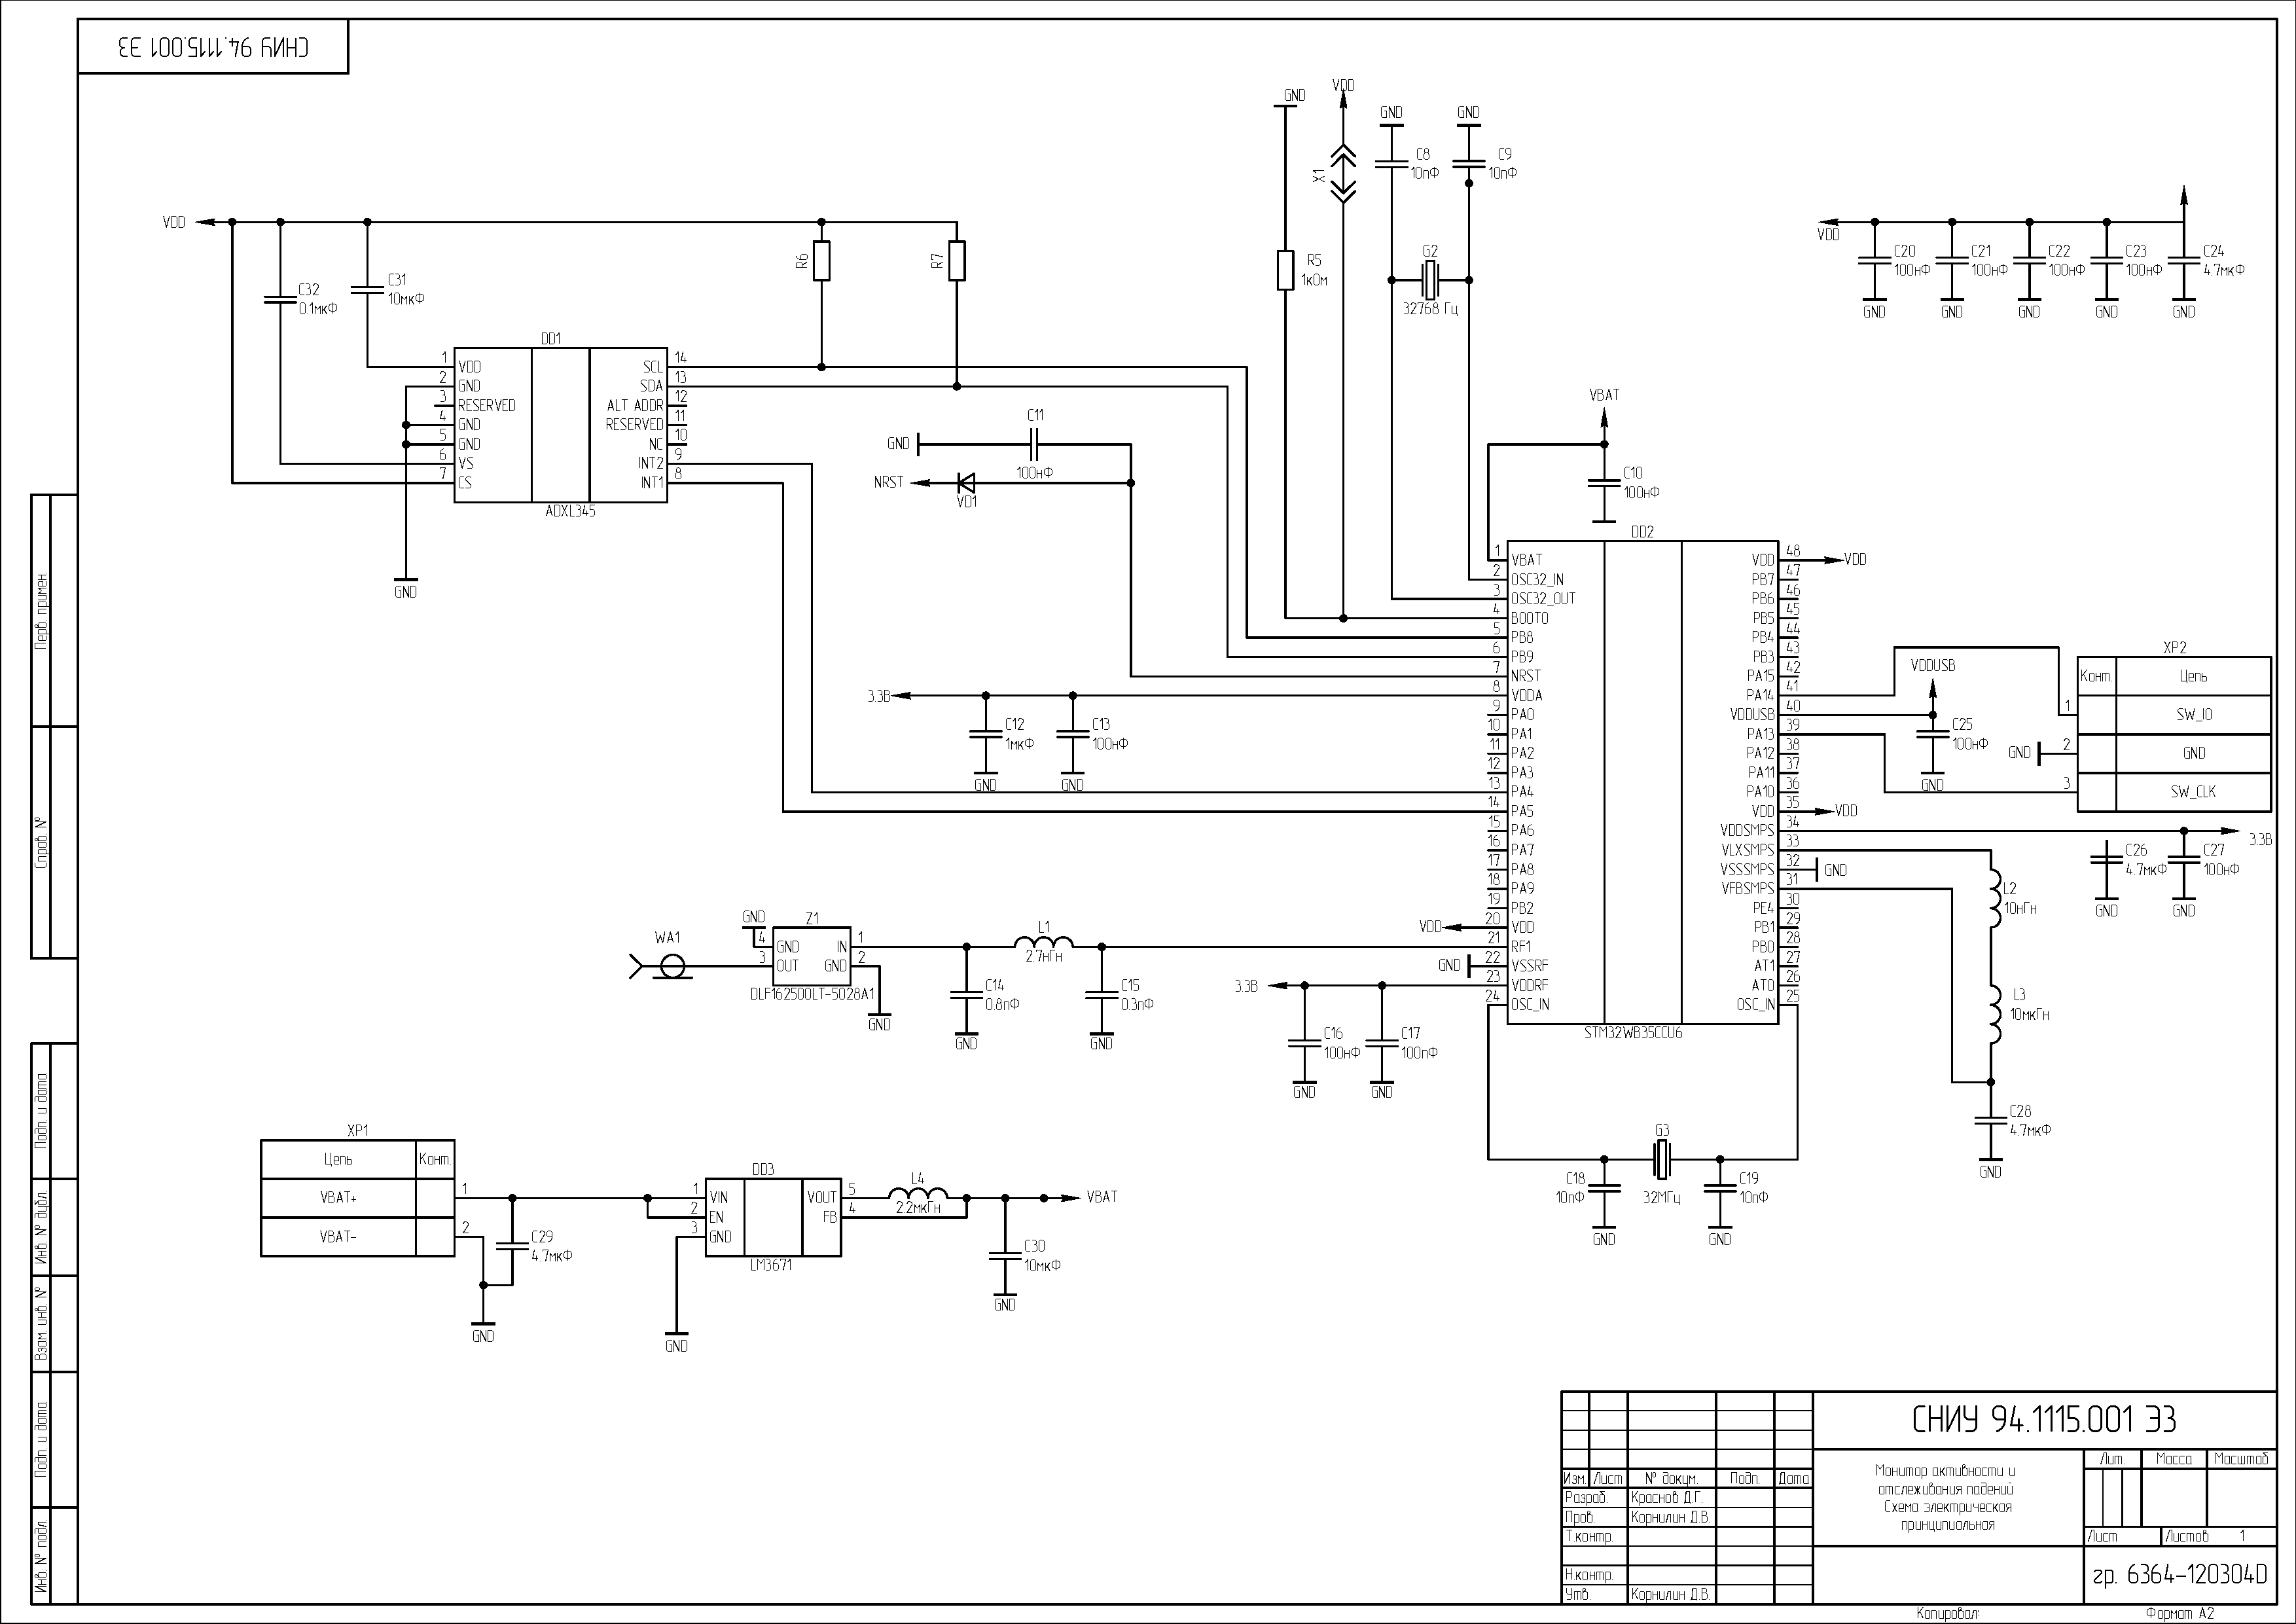
\includepdf{dg.pdf}
% текст в альбомной ориентации
% (таблица, рисунок, схема и т. п.)

% \
% это приложение

% \begin{sloppypar} % помогает в кириллическом документе выровнять текст по краям
\newpage % Так добавляется  новая страница

% \section*{ВВЕДЕНИЕ}%так объявляется новая глава. * означает, что эта глава не попадает в оглавление и не имеет номера.
% \addcontentsline{toc}{section}{\hspace{1mm}ВВЕДЕНИЕ} % эта строчка нужна, чтобы такую главу в оглавление все таки добавить, но без номера. Такие госты, что поделать.
% введение я вообще снес нахуй, так как не придумал, что там писать.
\section{МОДЕЛИРОВАНИЕ ДИФФЕРЕНЦИАЛЬНОГО УСИЛИТЕЛЯ С КОЭФФИЦИЕНТОМ УСИЛЕНИЯ 50} %Объявили начало раздела



\begin{table}[ht]
\caption{Расчет весомости параметров ПП}
\label{tab_weight}
\centering
    \begin{tabular}{|c|c|c|c|c|c|c|c|c|}
    \hline \multirow{2}{*}{Параметр $x_i$} & \multicolumn{4}{c|}{Параметр $x_j$} & 
        \multicolumn{2}{c|}{Первый шаг} & \multicolumn{2}{c|}{Второй шаг} \\
    \cline{2-9} & $X_1$ & $X_2$ & $X_3$ & $X_4$ & $w_i$ & 
        ${K_\text{в}}_i$ & $w_i$ & ${K_\text{в}}_i$ \\
    \hline $X_1$ & 1 & 1 & 1.5 & 1.5 &  0.31 & 19 & 0.32 \\
    \hline $X_2$ & 1 & 1 & 1.5 & 1.5 & 5 & 0.31 & 19 & 0.32 \\
    \hline $X_3$ & 0.5 & 0.5 & 1 & 0.5 & 2.5 & 0.16 & 9.25 & 0.16 \\
    \hline $X_4$ & 0.5 & 0.5 & 1.5 & 1 & 3.5 & 0.22 & 12.25 & 0.20 \\
    \hline \multicolumn{5}{|c|}{Итого:} & 16 & 1 & 59.5 & 1 \\
    \hline
    \end{tabular}
\end{table}





Во всех схемах были использованы операционные усилители общего назначения TL084. Их основные технические характеристики представлены в виде скриншотов из даташита на рисунках 1 и 2. 

\imgh{100mm}{Figures/1.png}{Схема ДУ на одном ОУ} 



\imghh{150mm}{Figures/2.png}{Фрагмент даташита на TL084} 


Для данной микросхемы коэффициент усиления по напряжению сигнала на постоянном токе – 200 В/мВ.


Для данной схемы \begin{math}K_\textup{ОУ}= 2*10^6\end{math} напряжение питания ±10 В. Выберем R1=R2=10 кОм. Рассчитаем оставшиеся резисторы, воспользовавшись следующей формулой: 

\begin{center}
\begin{math}K_\textup{d}= \frac{U_\textup{вых}}{U_2-U_1} = \frac{R3}{R1} \end{math} 
\end{center}


240.1k
244.755k

10.01k
10.2k



9.8k
9.99k





















Исходное задание звучит так:

\textit{Часы с индикацией минут и секунд на четырехзначном семисегментном индикаторе}
 
 
Схематически цифровое устройство, реализующее данный функционал можно изобразить с помощью блок-схемы, изображенной на рисунке \ref{ris:Figures/1.png}.

\imgh{160.5mm}{Figures/1.png}{Блок-схема секундомера} %можно так вставить изображение

Первый счетчик делит частоту встроенного в отладочную плату осциллятора со 100 МГц до 10 Гц, что соответствует периоду в одну миллисекунду.

Счетчик миллисекунд считает количество этих импульсов, считая от 0 до 9. Следующий счетчик считает так же от 0 до 9, что соответствует единицам секунд. 

Аналогично следующие два счетчика соответствуют десяткам секунд(считает от 0 до 5) и единицам минут(от 0 до 9).

Текущее значение каждого из счетчиков поступает на дешифратор, и затем на мультиплексор, который управляет катодами семисегментного индикатора. 
 
На аноды каждого из 4 индикаторов напряжение подается поочередно, с частотой незаметной глазу. Это обеспечивается с помощью отдельного делителя частоты. В качестве переменной величины для мультиплексора можно взять несколько  меняющихся битов какого-то вектора. Это и даст поочередное переключение 4 индикаторов.

Функция start--stop будет реализована с помощью кнопки без фиксации: по первому нажатию секундомер запускается, по второму останавливается, из любого этих состояний секундомер можно сбросить, иначе говоря, в одном состоянии счет времени осуществляется, в другом - нет, на индикаторе будут изображены те цифры, что были до остановки.

\subsection{Описание устройства с помощью VHDL} 
Описаннный в предыдущем пункте функционал реализуется с помощью следующего описания устройства на языке VHDL:
 \inputminted[
% frame=lines,%линия сверху и снизу блока кода
% framesep=15mm, % отступ между линией и кодом
baselinestretch=1, %интервал междустрочный
 % bgcolor=LightGray, %цвет фона
fontsize=\footnotesize, %размер шрифта
% linenos%нумерация строк
]
{VHDL}%язык программирования
{delitel.vhd}%файл с кодом(должен лежать в папке проекта)
Данный код полностью описывает логику требуемого устройства.


\subsubsection{Симуляция устройства} %Объявили начало раздела
Чтобы проверить, как полученное с помощью этого описания устройство работает, нужно запустить симуляцию. Для сокращения времени симуляции был изменен кусок кода со счетчиком, считающим до 10 миллионов.
\begin{minted} [
% frame=lines,%линия сверху и снизу блока кода
% framesep=15mm, % отступ между линией и кодом
baselinestretch=1, %интервал междустрочный
 % bgcolor=LightGray, %цвет фона
fontsize=\footnotesize, %размер шрифта
% linenos%нумерация строк
]{VHDL}
--if cnt=to_unsigned(10_000_000,28) then cnt <= (others => '0'); --считаем до 10M 
if cnt=to_unsigned(1000,28) then cnt <= (others => '0'); --считаем до 1000 
\end{minted}


Так же для симуляции необходимо создать файл симуляции (Test bench) SIMM.vhd на языке VHDL, содержимое которого можно увидеть ниже:


\inputminted[
% frame=lines,%линия сверху и снизу блока кода
% framesep=15mm, % отступ между линией и кодом
baselinestretch=1, %интервал междустрочный
% bgcolor=LightGray, %цвет фона
fontsize=\footnotesize, %размер шрифта
% linenos%нумерация строк
]
{VHDL}%язык программирования
{SIMM.vhd}%файл с кодом(должен лежать в папке проекта)

После запуска симуляции были получены временные диаграммы, изображенные на рисунках \ref{ris:Figures/2.png}, \ref{ris:Figures/3.png}, \ref{ris:Figures/4.png}, \ref{ris:Figures/5.png}, \ref{ris:Figures/6.png}, \ref{ris:Figures/7.png}%, \ref{ris:Figures/8.png}.


В начальный момент времени значения всех счетчиков не определены. При сбросе с помощью сигнала reset значения счетчиков обнуляются, после чего начинается счет посредством счетчика cnt. Досчитав до 1000(вообще он должен до 100 миллионов считать, но для симуляции ждать такое значение бессмысленно), счетчик сбрасывается, передавая импульс следующему счетчику, считающего миллисекунды. Он, в свою очередь считает до 9, и тактует счетчик единиц секунд, считающего до 9. Аналогично обстоит дело со следующими счетчиками. Так же, можно просмотреть момент, когда при нажатии кнопки start-stop запускается и останавливается счет времени.

\newpage
\imghh{160.5mm}{Figures/2.png}{Нулевой момент времени, сброс всех сигналов сигналом reset, начало отсчета счетчика cnt} 
\imghh{160.5mm}{Figures/3_2.png}{Остановка счета времени повторным нажатием кнопки start-stop } 
\imghh{160.5mm}{Figures/3.png}{Переключение счетчика миллисекунд при приходе импульса от делителя тактовой частоты cnt} 
\imghh{160.5mm}{Figures/4.png}{Переключение счетчика единиц секунд счетчиком миллисекунд}
\imghh{160.5mm}{Figures/5.png}{Переключение счетчика десятков секунд счетчиком единиц секунд} 
\imghh{160.5mm}{Figures/6.png}{Переключение счетчика единиц минут счетчиком десятков секунд} 
\imghh{160.5mm}{Figures/7.png}{Остановка счета нажатием кнопки start-stop -- значения счетчиков зафиксировались и не меняются} 
Таким образом, симуляцию можно считать успешной.


\section{Синтез цифрового устройства} %Объявили начало раздела
Для синтеза необходимо задать временные ограничения. Создаем файл временных ограничений, в котором нужно задать частоту тактового сигнала, в окне Primary Clocks. 

В результате синтеза была получена следующая схема(рисунок \ref{ris:Figures/sch.png})
\begin{landscape}
\imgh{250.5mm}{Figures/sch.png}{Синтезированная схема и сводка по времени} 
% текст в альбомной ориентации
% (таблица, рисунок, схема и т. п.)
\end{landscape}

\newpage
Система отмечает отсутствие ограничений Input и Output, а также группы no clock и unconstrained elements. Причина этого в том, что все счетчики тактируется выходным сигналом другого счетчика, который не указан в качестве тактового.

Так же на этом этапе необходимо указать внешние порты ввода-вывода для размещения схемы внутри ПЛИС. Сделать это нужно вручную, в соответствии со схемой, указанной в Board Reference Manual.


\imgh{160.5mm}{Figures/port.png}{Расположение портов ввода-вывода} 


\section{Реализация} %Объявили начало раздела
Следующий шаг разработки устройства – это реализация.
После завершения процесса реализации нужно проверить выполнение временных ограничений (Report Timing Summary)(рисунок \ref{ris:Figures/timing.png})
\imghh{160.5mm}{Figures/timing.png}{временная сводка после реализации} 
\section{Программирование ПЛИС} %Объявили начало раздела

Для программирования ПЛИС нужно выбрать Generate Bitstream на левой панели (Flow Navigator), а после завершения процесса открыть Hardware Manager, подключить кабель USB к отладочной плате (разъем PROG) и затем к компьютеру. Включить плату (переключатель POWER на плате), а также проверить правильность установки перемычек JP1 и JP2. 

В окне Hardware Manager необходимо выбрать ''Open Target'', а затем ''Auto Connect'' Если соединение будет успешным, надпись ''unconnected'' сменится на имя платы, появится кнопка ''Program Device''. При нажатиии на нее нужно выбрать отладочную плату, а затем файл с битовым потоком (с расширением
.bit) -- ''Bitstream file'' . Нажать ''Program''.

\section{Проверка функционирования устройства на отладочной плате} %Объявили начало раздела
После завершения программирования устройства была произведена проверка его работоспособности, в результате которой было выяснено, что устройство работает корректно. Функции, возложенные на кнопки reset, start-stop правильно работают, все описанные и требуемые заданием функции устройства работают.

\end{sloppypar}
% осн часть


%\begin{landscape}
% текст в альбомной ориентации
% (таблица, рисунок, схема и т. п.)
%\end{landscape}

% \likechapter{Вступление}
% ебал все в рот



%\input{RefProject-App}% приложение








\end{document}